\documentclass[b5paper,opensource]{./template/qyxf-book}

\usepackage{subcaption}
% 添加水印的宏包
\usepackage{draftwatermark}
\SetWatermarkText{钱院学辅}
\SetWatermarkLightness{0.9}
\SetWatermarkScale{0.9}

% 基本不需要改动
\title{大物题解}
\subtitle{Key to Universal Physics}
\author{钱院学辅大物编写小组}
\typo{钱院学辅排版组}
\date{\today}
\version{v1.0}
\sourcepage{\url{https://github.com/qyxf/Tutorials/}}

% 这里可以自定义一些命令
\newcommand{\di}[1]{\mathrm{d}#1}
\newcommand{\p}[2]{\frac{\partial #1}{\partial #2}}
\newcommand{\pp}[2]{\frac{\partial ^2 #1}{\partial #2 ^2}}
\newcommand{\dy}[2]{\frac{\di{#1}}{\di{#2}}}
\newcommand{\ddy}[2]{\frac{\mathrm{d} ^2 #1}{\mathrm{d} #2 ^2}}
\newcommand{\zbj}[4]
{
	\draw (0,0) node[below left] {$ O $};
	\draw [->] (#1,0) -- (#2,0) node[right] {$ x $};
	\draw [->] (0,#3) -- (0,#4) node[right] {$ y $};
}


\begin{document}

\maketitle 
\tableofcontents

%% 对于章节编写,可以不加封面和目录
\chapter{运动学}  % 使用章节\chapter{}来做一级标题
\section{选择题}  % 选择题、填空题和解答题使用\section{}

\exercise{1}A  % 题号使用这个命令,会自动生成标记,注记后写主要答案

\solve  % 解答使用这个命令,解答与题号之间空一行
如图1.1,对M,在x方向上:
\begin{equation*} % 单行公式可以使用这个命令
N\cos\theta=Ma_a\text{(M对地)}
\end{equation*}
如图1.2,对m,以M为参考系,m受一惯性力,合加速度沿二者接触面。沿x,y方向分解: % 大段文字需要写在公式外面
\begin{gather}
mg-N\cos\theta=ma_r\sin\theta \\
ma_a+N\sin\theta=ma_r\cos\theta
\end{gather}
将(1)代入(2),由(2)(3)可联立解得:
\[
a_r=\dfrac{(M+m)g\sin\theta}{M+m{\sin\theta}^2}
\]

\centerline{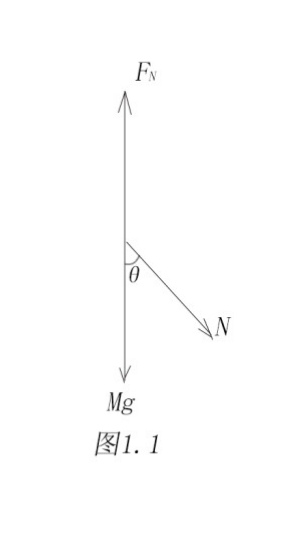
\includegraphics[width=10em,height=15em]{Chp1_illus1.png}  % 这个命令是对某些行居中
\quad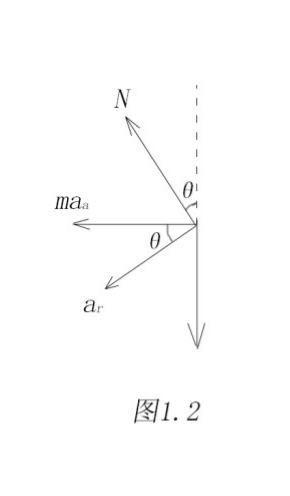
\includegraphics[width=10em,height=15em]{Chp1_illus2.png}}

%% 空一行开始下一个题目
\exercise{2}B

\solve 如图1.3,$u=v\cos\theta$,v不变而$\theta$增大,需要u减小。
\centerline{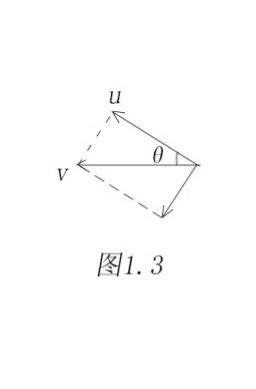
\includegraphics[width=6.5em,height=10em]{Chp1_illus3.png}}

\exercise{3}A

\solve 匀速圆周运动的速度、加速度(受力)均是大小不变、方向时刻变化。
注意一个矢量为常量包括大小和方向两个方面。否则就是变化的量。

\exercise{4}B

\solve 以前面的货车为参考系,货车静止,火车速率为$v_1-v_2$,加速度为$a$(反向),那么火车最多前进$s=\dfrac{{(v_1-v_2)}^2}{2a}$。要求$d>s$,故选B。或采用地面参考系的追逐问题法,计算从$v_1$减速到$v_2$两车走过的距离之差:
\[
s=\dfrac{{v_1}^2-{v_2}^2}{2a}-v_2\cdot \dfrac{v_1v_2}{a}=\dfrac{{(v_1-v_2)}^2}{2a}
\]

\exercise{5}C

\solve 两次求导得:$a=30t\neq$常数而大于零。

\exercise{6}B

\solve 求导得:$v=8t-6t^2,a=8-12t$。
令$y=0\Rightarrow t=0\text{(舍去)或}2$,代入得结果。

\exercise{7}B

\solve 物体做匀加速直线运动。

\begin{gather*}
s=\dfrac{b}{\cos\alpha},a=g\sin\alpha\\
t=\sqrt{\dfrac{2s}{a}}=\sqrt{\dfrac{4b}{g\sin(2\alpha)}}
\end{gather*}

$t$最小时,$\sin(2\alpha)$最大,$\alpha=45^\circ$。

\exercise{8}B

\solve 类比从静止出发的匀加速直线运动。$t=\dfrac{2\cdot 2\pi}{\beta}$

\exercise{9}B

\solve 曲线的定义:“\textit{动点运动方向连续变化的轨迹}”
\footnote{来源:汉典网http://www.zdic.net/c/2/111/299079.htm}
。A,C的反例:匀速圆周运动。

\exercise{10}D

\solve 反例:平抛运动

\section{填空题}
\exercise{11} 0\qquad2g

\solve 设A、B质量为m。抽走C之前,弹簧中的弹力大小为mg。撤去C时,弹簧长度未突变,弹力不变,A受合力为0;支持力则消失。故
\begin{gather}
a_A=0 \\
a_B=\dfrac{mg+mg}{m}=2g\quad(\text{竖直向下})
\end{gather}

\exercise{12} $\dfrac{25}{12}\pi\ rad/s^2$ \qquad$\dfrac{24}{5}s$

\solve 简单公式应用
\begin{gather*}
\theta=60\times2\pi=120\pi\\
\beta=\dfrac{\omega_2^2-\omega_1^2}{2\theta}=\dfrac{25}{12}\pi\ rad/s^2\\
\delta t=\dfrac{\omega_2-\omega_1}{\beta}=\dfrac{24}{5}s
\end{gather*}
\exercise{13} $m(\sin\theta-\omega^2l\sin\theta\cos\theta)$

\solve
\begin{figure}[htbp]  % 可以使用figure来导入图片
	\centering
	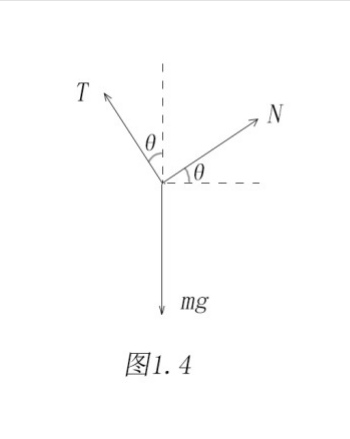
\includegraphics[width=15em, height=15em]{Chp1_illus4.png}
	\caption{练习13}
	\label{fig:c1}
\end{figure}
如图\ref{fig:c1},在x,y方向上分解受力,得  % 引用图片使用\ref
\begin{gather*}
% \text{:如图1.4,在x,y方向上分解受力,得 }\\		% 不要这样写,格式会乱!!!
T\sin\theta-N\cos\theta=m\omega^2l\sin\theta\\
T\cos\theta+N\sin\theta=mg\\
\end{gather*}
联立可解得T、N的大小。

\exercise{14} $2\sqrt{\dfrac{r}{g}}$ \qquad $2\sqrt{\dfrac{r}{g}}$

\solve
\begin{gather*}
\text{设弦与PC的夹角为}\theta,\text{则有}\\
s=2r\cos\theta,a=g\cos\theta\\
t=\sqrt{\dfrac{2s}{a}}=2\sqrt{\dfrac{r}{g}}
\end{gather*}

\exercise{15} $4\sqrt{5}m/s$ \qquad $16m/s^2 $ 

\solve
\begin{gather*}	
\text{抛物线的切线方向即为质点的速度方向,且}x=4t\\
\therefore \dfrac{v_y}{v_x}=\dy{y}{x}=x\Rightarrow v_y=4x=16t\\
\therefore t=2\text{时,}v_y=8\mathrm{m/s},
v=\sqrt{{v_x}^2+{v_y}^2}=4\sqrt{5}\mathrm{m/s}\\
v_x\text{不变,}a=a_y=\dy{v_y}{t}=16\mathrm{m/s^2}
\end{gather*}

\exercise{16} 长度、质量、时间\par

\solve 见课本,解答略。\\

\exercise{17} 3\quad 3\quad 6

\solve x分别对t求一阶两阶导即是v、a,由图像即可判断其正负号。\\

\exercise{18} $y={(x+5)}^3$

\solve
\begin{gather*}\text{由题,}x=2t-5\Rightarrow 2t=x+5\\
\text{代入}y=8t^3={(2t)}^3\text{,消去t即可}
\end{gather*}	

\exercise{19} $\dfrac{1}{2}g$\qquad 竖直向下%\par  这里不用写\par

\solve  初始时受力平衡,两根弹簧上力均为$\dfrac{1}{2}mg$;一根断掉后,向上的力减半,则小球受的合力是$\dfrac{1}{2}mg$,竖直向下。

\exercise{20} 9m/s 
\solve
\begin{gather*}\text{(SI)} x=3t+6t^2-2t^3\xrightarrow{\text{求导}}v=3+12t-6t^2\\
\xrightarrow{\text{求导}}a=12-12t\\\
令a=0\ \text{解得}\ t=1\xrightarrow{\text{代入得}} v(1)=9\mathrm{m/s}
\end{gather*}


\section{计算题}
%21,22,24题对原作者代码有改动
\exercise{21}

\solve 由图知:
\begin{gather*}
\tan\alpha=\dfrac{|\vec{a}_n|}{|\vec{a}_\tau|}=\dfrac{\dfrac{v^2}{R}}{\dy{v}{t}}\\
\therefore \dy{v}{t}\frac{1}{v^2}=\frac{1}{R\tan\alpha}
\end{gather*}
积分得:
\begin{equation*}
-\frac{1}{v}=\frac{1}{R\tan\alpha}t+C	
\end{equation*}
代入 $ t=0,v=v_0 $
\begin{gather*}
\therefore \frac{1}{v_0}-\frac{1}{v}=\frac{1}{R\tan\alpha}t \\ \text{即}v=\frac{v_0R\tan\alpha}{\tan\alpha-v_0t}
\end{gather*}

\exercise{22}

\solve 
\begin{gather*}
\vec{v}=\dy{s}{t}\vec{\tau}=(c+2dt)\vec{\tau}\\  
\vec{a}_n=\frac{v^2}{R}\vec{n}=\frac{(c+2dt)^2}{R}\vec{n}\\
\vec{a}_\tau=\dy{v}{t}\vec{\tau}=2d\vec{\tau}\\
\text{令}|\vec{a}_n|=|\vec{a}_\tau|,
\text{则}\frac{(c+2dt)^2}{R}=2d\\
\therefore t_1=\frac{\sqrt{2dR}-c}{2d}\left(t_2=\frac{-\sqrt{2dR}-c}{2d}<0\text{,舍去}\right)\\
\therefore\text{要使t}\geqslant\text{0,条件为}\sqrt{2dR}-c\geqslant0,\text{即}2dR\leqslant c^2
\end{gather*}

\exercise{23}
\begin{gather*}
-kx=a=\dy{v}{t}=\dy{v}{x}\cdot \dy{x}{t}=\dy{v}{x}\cdot v\\
\text{分离变量,积分得:}-\dfrac{1}{2}kx^2=\dfrac{1}{2}v^2+C_1\\
\text{令}C=2C_1,\text{则}-kx^2=v^2+C\\
\text{代入 }x=x_0,v=v_0\text{\,得:  }C=-(kx_0^2+v_0^2)\\
\text{整理得:  }v=\pm\sqrt{kx_0^2+v_0^2-kx^2}
\end{gather*}

\exercise{24}

\solve
(1)
\begin{align*}
v&=10\left(1-\frac{t}{5}\right)\\
&=-2t+10\\
\dy{x}{t}&=-2t+10
\end{align*}
\vspace{-2.5em}
\begin{gather*}
\text{积分得:}x=-t^2+10t+c\\
\text{代入}t=0,x=0,\quad \therefore x=-t^2+10t\\
\text{代入}t=10s\\
\therefore x=0.\quad
\therefore\text{坐标为}0\\
\end{gather*}

(2)
\begin{gather*}
\text{令}x=10m,\therefore t^2-10t+10=0\\
\therefore t=5\pm\sqrt{15}s\\
\text{令}x=-10m,\therefore t^2-10t+10=0\\
\therefore t=5+\sqrt{35}(5-\sqrt{35}<0,\text{舍去})\\
\therefore\text{时刻为}5-\sqrt{15}\ s,5+\sqrt{15}\ s\text{或}5+\sqrt{35}\,s\\
\end{gather*}

(3)
\begin{gather*}
\text{令}v=0,\therefore t=\ 5s\\
\therefore t\in[0,5],\quad s=x=-t^2+10t\\
t\in[5,+\infty),\quad s=s(5)+[s(5)-x]=25\\+[25-(-t^2+10t)]
=t^2-10t+50\\
\therefore s=
\begin{cases}
-t^2+10t,&t\in[0,5)\\
t^2-10t+50,&t\in[5,+\infty)
\end{cases}
\end{gather*}

\chapter{动量和冲量}
\section{选择题}

\exercise{1}C
	
	\solve
质点沿力方向位移为零。$\therefore A=0$.\\

\exercise{2}B

\solve
$B$离开$A$时为弹簧恢复原长的时刻(该时刻之后,$A$受到弹簧拉力,加速度为负,$v_A<v_B$.)\par
此时$v_A=v_B$.由动能定理:
\begin{align*}
\frac{1}{2}mv_A^2+\frac{1}{2}mv_B^2-0=\frac{1}{2}kd^2\\
\therefore{}E_B=\frac{1}{2}mv_B^2=\frac{1}{4}kd^2
\end{align*}

\exercise{3}C

\solve
对$\vec{r}$求导:
\begin{align*}
\vec{v}&=\frac{\di{\vec{r}}}{\di{t}}\\
&=-\frac{2\pi}{T}A\sin\frac{2\pi t}{T}\vec{i}+\frac{2\pi}{T}B\cos\frac{2\pi t}{T}\vec{j}
\end{align*}
\par$t=0$时,
\begin{align*}
v_1&=\sqrt{v_{x1}^2+v_{y1}^2}\\
&=\sqrt{0^2+\left(\frac{2\pi}{T}B\right)^2}=\frac{2\pi}{T}B
\end{align*}
\[\therefore{}E_{k1}=\frac{1}{2}mv_1^2=\frac{2m\pi^2}{T^2}\left(B^2\right)\\\]
\par$t=\frac{T}{4}$时,
\begin{align*}
v_2&=\sqrt{v_{x2}^2+v_{y2}^2}\\
&=\sqrt{\left(-\frac{2\pi}{T}A\right)^2+0^2}=\frac{2\pi}{T}A
\end{align*}
\begin{gather*}
\therefore{}E_{k2}=\frac{1}{2}mv_2^2=\frac{2m\pi^2}{T^2}\left(A^2\right)\\
\therefore\Delta{}E_k=\frac{2\pi^2}{T^2}(B^2-A^2)
\end{gather*}

\exercise{4}D

\solve
由动量定理:
\[0=m_1v_1-m_2v_2\]
\[\therefore{}v_2=\frac{m_1}{m_2}v_1\]\par
由机械能守恒:
\begin{align*}
E_p &=\frac{1}{2}m_1v_1^2+\frac{1}{2}m_2v_2^2\\
&=\frac{m_1v_1^2+\frac{m_1^2v_1^2}{m_2}}{2}\\
&=\frac{m_1v_1^2\left(m_1+m_2\right)}{2m_2}
\end{align*}
\exercise{5}B

\solve
(2):既然小车能在水平面上停止,说明水平面是粗糙的,有摩擦力做功。因此不满足机械能守恒。\par
(4):重力做正功,摩擦力做负功,符号相反。\\
\exercise{6}D

\solve
弹簧上任意一点弹力相同,记为N。截去一半后,伸长量缩短了一半,而弹力不变,因此k变为原来的两倍。\par
并联在一起后,每一根弹簧受力为原先的一半。由$F=kA$,伸长量为原来的$\frac{1}{4}$。\par
写成数学式子如下:
\begin{align*}
E_k &=2\times\left(\frac{1}{2}k'A'^2\right)\\
&=\left(2k\right)\times\left(\frac{1}{4}A\right)^2\\
&=\frac{1}{8}kA^2
\end{align*}
\exercise{7}D

\solve
物体沿重力方向的位移为负,因此重力做负功。其它选项,物体沿推力方向有位移,因此推力做功,A错误;推力功与摩擦力做的功和重力做的功之和等值反号,因此B错误。\\
\exercise{8}C

\solve
若合外力的冲量为0,则由冲量定义$\vec{I}=\int_{t1}^{t2}\vec{F}\di{t}$知,$\vec{F}=\vec{0}$,因此合外力做的功为0。其它选项,AD可举匀速圆周运动的反例;对于B,合外力不为0,必有加速度,而质量不改变,因此$\vec{v}$必然改变,即动量必改变。\\
\exercise{9}B

\solve 
由动能表达式$E_k=\frac{p^2}{2m}$,在动量相同的情况下,质量越大,动能越小,因此选B\\
\exercise{10}A

\solve
设小球重力为$G$,弹簧弹性系数为$k$,则$G=kd$,再设最低点时弹簧伸长$h$。以弹簧原长的高度为基准,释放前和最低点为始末态,应用机械能守恒:
\[Gh=\frac{1}{2}kh^2\]
解得$h=2d$

\section{填空题}

\exercise{11}$31J$

\solve
\[A=\int_{0.5}^{1}F\di{x}=\int_{0.5}^{1}(52.8x+38.4x^2)\di{x}=31(J)\]
\exercise{12}$24J$ $4m/s$

\solve
\[A=\int_{1}^{4}F\di{x}=\int_{1}^{4}(3+2x)\di{x}=24(J)\]
\[\text{由动能定理:}\frac{1}{2}mv^2=24,\quad \therefore v=4(m/s)\]
\exercise{13}$\frac{GMm}{6R}$ \qquad $-\frac{GMm}{3R}$

\solve
\begin{gather*}
\text{卫星运动的向心力由万有引力提供,}\therefore m\frac{v^2}{3R}=G\frac{Mm}{(3R)^2}\\
\therefore E_k=\frac{1}{2}mv^2=\frac{GMm}{6R}\\
\text{由引力势能公式:}E_p=-\frac{GMm}{r}=-\frac{GMm}{3R}
\end{gather*}
\exercise{14}1296

\solve
\begin{gather*}
\text{由牛顿第二定律:}F=ma,\qquad t^2=2a=2\ddy{x}{t},\\
\text{再由初始条件}t=0,x=0\text{且}v=0, \text{解得}x=\frac{1}{24}t^4\\
\text{由此可知}x=54m\text{时}, t=6s\\
A=\int_{0}^{6}F\di{x}=\int_{0}^{6}t^2\di{(\frac{1}{24}t^4)}\\
\therefore A=1296J
\end{gather*}
\exercise{15}$19.8m/s$

\solve
(小行星的物理量下标为1)
\begin{gather}
\text{向心力由万有引力提供,}\therefore m\frac{v_1^2}{R_1}=G\frac{Mm}{R_1^2}\notag\\
\text{将}M=\frac{4}{3}\pi R^3\rho\text{代入,得}v_1=\sqrt{G\frac{4}{3}\pi\rho R_1^2}\\
\text{由地球上重力为}g=9.8m/s,mg=G\frac{Mm}{R_2^2}\notag\\
\therefore g=G\frac{4}{3}\pi R_2\rho.\text{则}G\frac{4}{3}\pi\rho=\frac{g}{R_2}\notag\\
\text{代入(1),}v_1=\sqrt{\frac{gR_1^2}{R_2}}\approx19.8(m/s)\notag
\end{gather}
\exercise{16}$\sqrt{\frac{2Mgh}{m+M}}$ \qquad $\frac{m^2gh}{M+m}$

\solve
\begin{gather}
\text{由动量定理:}mv_1=Mv_2\\
\text{由机械能守恒:}mgh=\frac{1}{2}mv_1^2+\frac{1}{2}Mv_2^2\\
\text{联立(1)(2)解得:}v_1=\sqrt{\frac{2Mgh}{m+M}}\notag\\
v_2=\sqrt{\frac{2m^2gh}{(m+M)M}}\notag\\
\text{由动能定理知,物块对滑道做的功就是滑道动能改变量}\notag\\
\text{即}\frac{1}{2}Mv_2^2=\frac{m^2gh}{M+m}\notag
\end{gather}
\exercise{17}第i个质点所受合力做的功(类似说法均正确)\\

\exercise{18}1m/s \qquad 200J

\solve
船员用200N的力拉绳子,由牛顿第三定律,绳子也给船员(和船)200N的拉力。以人和船为对象应用牛顿第二定律,解得:
\[a=\frac{F}{m}=0.5m/s^2\]
因此第2秒末速率为1m/s,增加的动能就是
\[E_k=\frac{1}{2}mv^2=\frac{1}{2}\times400\times1^2=200(J)\]
\exercise{19}$\left(\frac{1}{r_2}-\frac{1}{r_1}\right)GMm$

\solve 
\begin{gather*}
\text{由机械能守恒,}0+E_{p1}=E_k+E_{p2}\\
\therefore E_k=E_{p2}-E_{p1}=\left(\frac{1}{r_2}-\frac{1}{r_1}\right)\\
\text{以两个质点为系统,仅有万有引力(内力)做功,因此由质点系动能定理:}\\
A=E_k=\left(\frac{1}{r_2}-\frac{1}{r_1}\right)GMm
\end{gather*}
\exercise{20}$0.8\sqrt{2}$

\solve
\centering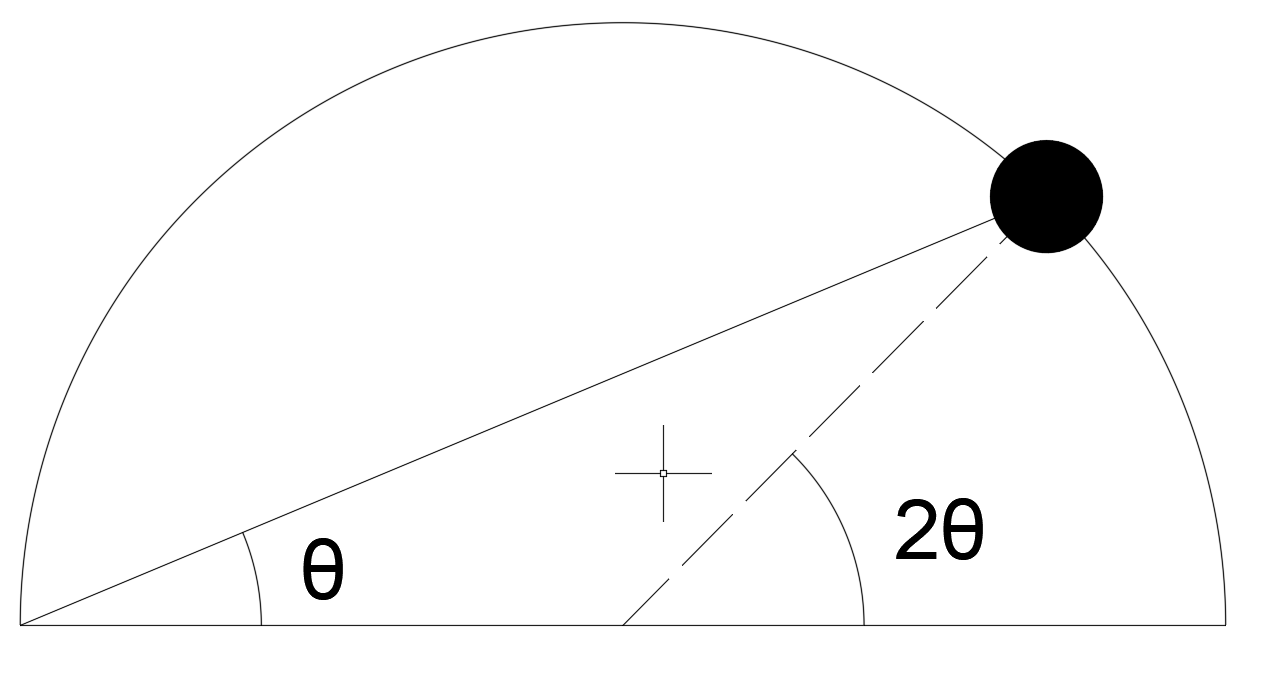
\includegraphics[height=100pt]{Chp2_illus1.png}\\
图1
\begin{align*}
A	&=\int_{\theta=0}^{\theta=\frac{\pi}{4}}{vec{F}}\cdot\di{vec{x}}\\
&=\int_{\theta=0}^{\theta=\frac{\pi}{4}}F\di{x}\cos\left(\frac{\pi}{2}-\theta\right)\\
&=\int_{0}^{\frac{\pi}{4}}k(2R\cos\theta-0.1)\times\di{(R\times 2\theta)}\times\sin\theta\\
&=\int_{0}^{\frac{\pi}{4}}(-4R^2k\cos\theta+0.2Rk)\di{(\cos\theta)}\\
&=-2R^2k\cos^2\theta+0.2Rk\cos\theta\left.\right|_0^{\frac{\pi}{4}}\\
&=-2\times 0.2^2\times 40\times({\frac{\sqrt{2}}{2}}^2-1^2)+0.2\times 0.2\times 40\times(\frac{1}{2}-1)\\
&=0.8\sqrt{2}
\end{align*}
\raggedright
\section{计算题}
\exercise{21}

\solve (1)
\begin{gather*}
\Delta l=\frac{F}{k}\\
E_p=\frac{1}{2}k(\Delta l)^2=\frac{F^2}{2k}\\
\text{由机械能守恒,}E_{kright}-0=E_p-0\\
\therefore\frac{1}{2}Mv_{\text{右}}^2=\frac{F^2}{2k}\\
\therefore v_{\text{右}}=\frac{F}{\sqrt{Mk}}
\end{gather*}
(2)
\begin{gather*}
\text{由受力分析知,}a_{\text{左}}=a_{\text{右}},\quad\text{即}\dy{v_{\text{左}}}{t}=-\dy{v_{\text{右}}}{t}\\
\text{两边积分:}\therefore v_{\text{左}}=-v_{\text{右}}+c\\
\text{代入刚恢复原长时:}v_{\text{左}}=0,v_{\text{右}}=\frac{F}{\sqrt{Mk}}\\
\therefore v_{\text{左}}+v_{\text{右}}=\frac{F}{\sqrt{Mk}}\\
\therefore\text{当}v_{\text{左}}=v_{\text{右}}\text{时},v'_{\text{左}}=v'_{\text{右}}=\frac{F}{\sqrt{2Mk}}\\
\text{由机械能守恒:}\\
0+\frac{1}{2}M(v_{\text{右}})^2=\frac{1}{2}k(\Delta l)^2+\frac{1}{2}M(v'_{\text{左}})^2+\frac{1}{2}M(v'_{\text{右}})^2\\
\therefore\Delta l=\pm\sqrt{\frac{M\left(\frac{F^2}{Mk}-2\times\frac{F^2}{4Mk}\right)}{k}}\\
=\pm\frac{\sqrt{2}}{2}\frac{F}{k}\\
\text{即伸长或压缩}\frac{\sqrt{2}}{2}\frac{F}{k}
\end{gather*}

\exercise{22}

\solve
记x为链条右端的位移,l为桌边链条的长度。
\begin{align*}
dA	&=F\cdot\di{x}\\
&=F\di{x}
\end{align*}
链条被匀速拉起,可知$F=G$
\begin{align*}
F	&=G=M'g\\
&=\frac{l}{L}Mg
\end{align*}
由几何意义,$\di{x}=-\di{l}$
\begin{align*}
\therefore A&=\int_{\frac{L}{3}}^{0} -\frac{l}{L}Mg\di{l}\\
&=\frac{Mg}{2L}l^2\left.\right|_{0}^{\frac{L}{3}}\\
&=\frac{MgL}{18}
\end{align*}
如果有摩擦力f,则
\begin{align*}
\di{A}	&=F'\di{x}\\
F'		&=G+f=\frac{l}{L}Mg+\mu\left(\frac{L-l}{L}Mg\right)\\
&=\frac{Mg}{L}[\mu L+(1-\mu)l]\\
\therefore A&=\int_{\frac{L}{3}}^{0} -\frac{Mg}{L}[\mu L+(1-\mu)l] \di{l}\\
&=\frac{Mg}{L}\left(\mu Ll+\frac{1-\mu}{2}l^2\right)\left.\right|_{0}^{\frac{L}{3}}\\
&=\frac{Mg}{L}\left(\frac{\mu}{3}L^2+\frac{1-\mu}{18}L^2\right)\\
&=MgL\frac{5\mu +1}{18}
\end{align*}

\exercise{23}

\solve \centering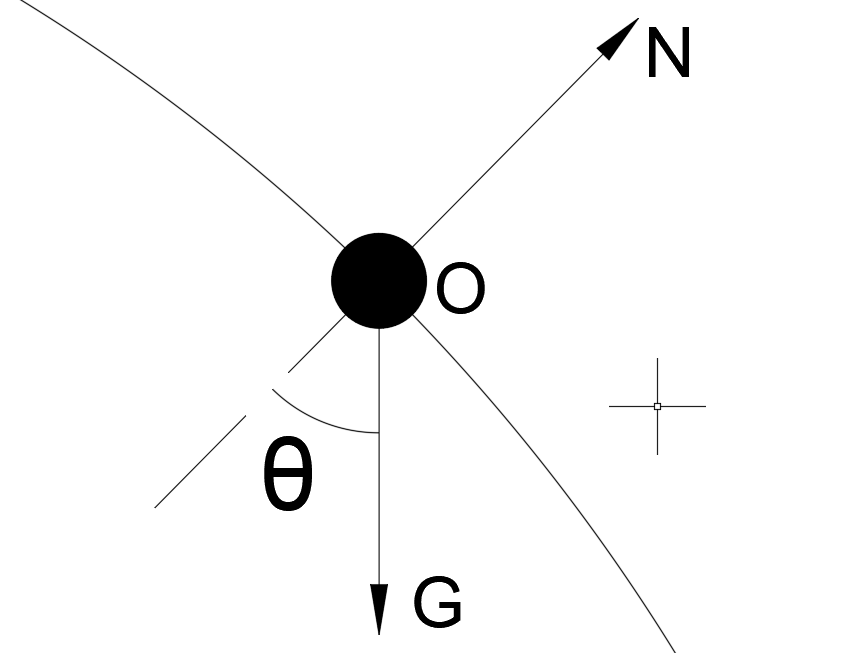
\includegraphics[height=100pt]{Chp2_illus2.png}\\
图2\\
\raggedright 由图2,对小球应用牛顿第二定律:
\[m\frac{v^2}{R}=mg\cos\theta-N\]
\centering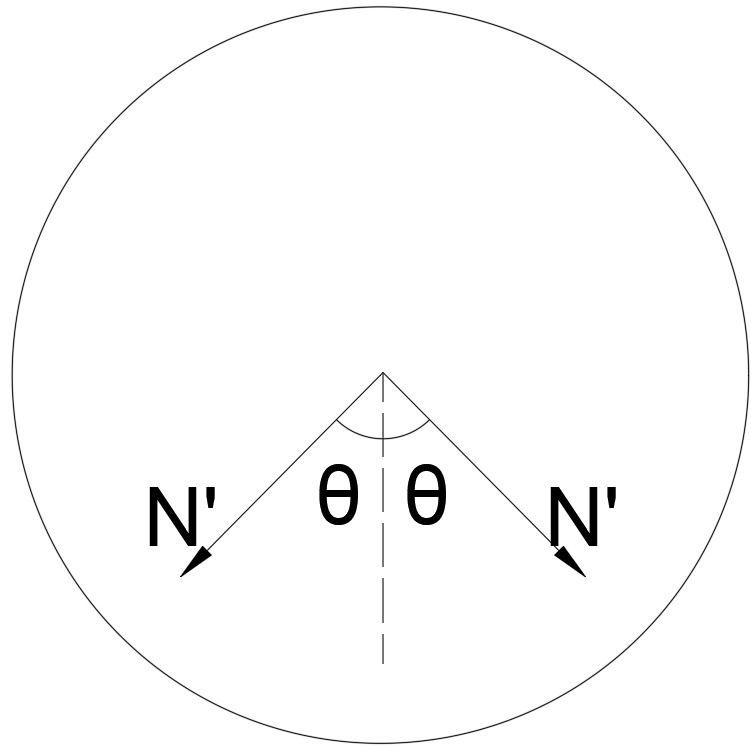
\includegraphics[height=100pt]{Chp2_illus3.png}\\
图3\\
\raggedright 由受力分析知,圆环竖直方向受力F为:
\begin{gather*}
F=(N'+N')\cos\theta=2N\cos\theta
\text{当}\theta\in[0,\frac{\pi}{2}]\text{时},\cos\theta>0\\
\therefore\text{当}N<0\text{时},F\text{向上,圆环上升}\\
\therefore N=mg\cos\theta-m\frac{v^2}{R}<0\\
\text{由机械能守恒(见图4):}\frac{1}{2}mv^2=mgh=mg(1-\cos\theta)R\\
\end{gather*}
\centering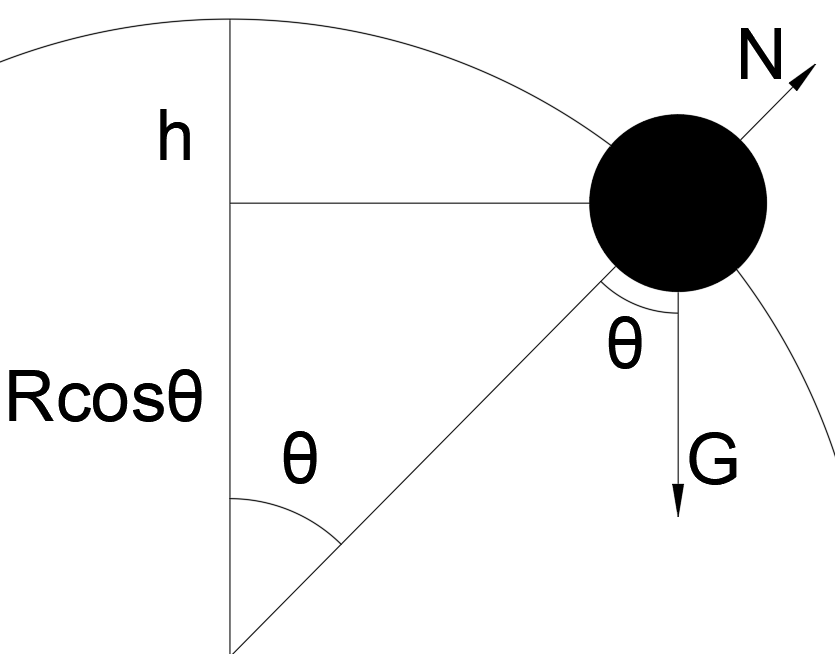
\includegraphics[height=100pt]{Chp2_illus4.png}\\
图4
\begin{gather*}
\text{代入,}\therefore mg\cos\theta-2mg(1-\cos\theta)<0\\
\therefore 3\cos\theta<2,\quad \theta>\arccos\frac{2}{3}\\
\text{即当}\theta>\arccos\frac{2}{3}\text{时,圆环会上升}
\end{gather*}
\raggedright

\exercise{24}

\solve
\begin{gather*}
T_1\text{提供}G1+G2\\
\therefore k_1\Delta l=(m_1+m_2)g\\
\Delta l=\frac{(m_1+m_2)g}{k_1}\\
\text{由机械能守恒:}\\
-mgx+\frac{1}{2}k_1(\Delta l+x)^2+\frac{1}{2}m_1v^2=0+\frac{1}{2}k_1(\Delta l)^2+0
\end{gather*}
\begin{align*}
\therefore v&=\sqrt{\frac{-kx^2-2(k_1\Delta l-m_1g)x}{m_1}}\\
&=\sqrt{-\frac{k_1}{m_1}x^2-\frac{2m_2g}{m_1}x}
\end{align*}
利用二次函数最大值为$\frac{4ac-b^2}{4a}$的性质:
\begin{align*}
v_{max}	&=\sqrt{\frac{0-\frac{4m_2^2g^2}{m_1^2}}{4\left(-\frac{k_1}{m_1}\right)}}\\
&=\sqrt{\frac{m_2^2g^2}{m_1k_1}}=\frac{0.3\times 9.8}{\sqrt{0.5\times 8.9\times 10^4}}\\
&=0.0139(m/s)
\end{align*}

\end{document}
